\section{Cele pracy}
\label{sec:cel}

Praca skupia się wokół symulacji badania metalowych prętów przy pomocy fal prowadzonych. Symulacja ma za zadanie wyznaczyć sygnał zwrotny, dla nadanego sygnału za pomocą np. przetwornika piezoelektrycznego, w przypadku badania puls-echo. Fale prowadzone podlegają dyspersji, więc sygnał powrotny jest silnie zniekształcony w stosunku do nadanego. Algorytmy, które pozwolą skompensować dyspersję są kolejnym aspektem branym pod uwagę przy symulowaniu przebiegu sygnału.

Pomysł na tego typu symulację wziął się z problemu badania kotw stropowych przedstawionego w [!!!]. Jeśli wykorzystamy metalowe pręty aby wzmocnić strop tunelu i mamy do nich dostęp wyłącznie od strony czoła, to możliwości sprawdzania stanu tych prętów jest mocno ograniczony. Rysunek \ref{fig:kotwy} przedstawia widok tunelu i kotw stropowych. Sposobem na diagnostykę kotw, może być właśnie zastosowanie fal prowadzonych. 

\begin{figure}[h]
\centering
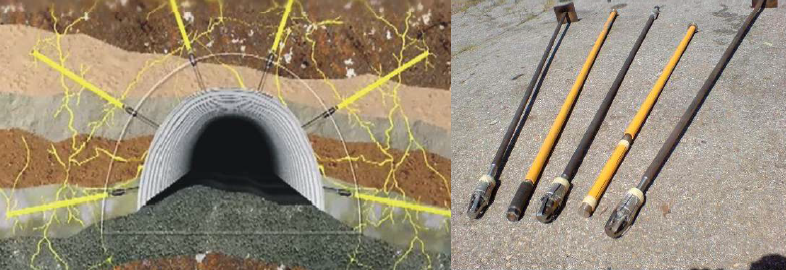
\includegraphics[width=14cm]{Zdjecia/1/kotwy}
\caption{Zastosowanie kotw do wzmacniania stropu oraz różne rodzaje kotw}
\label{fig:kotwy}
\end{figure}

\vspace{5mm}

Aby dać możliwość symulacji badania pręta, program musi zapewniać następujące funkcjonalności:
\begin{enumerate}
  \item Możliwość wyboru sygnału wejściowego
  \item Możliwość wyznaczenia modelu matematycznego pręta
  \item Możliwość wyznaczenia sygnału zwrotnego z uwzględnieniem parametrów pręta
  \item Możliwość wyznaczenia krzywych dyspersji dla pręta o zadanych właściwościach materiałowych
  \item Możliwość kompensacji dyspersji sygnału wyjściowego.
\end{enumerate}

\vspace{5mm}

Dodatkowo program daje możliwość wyznaczania krzywych wzbudzalności dla pręta i symulacji badania w układzie samowzbudnym (efekt sing-around).



















